
% federated-learning.tex

\documentclass[dvipdfmx,notheorems,t]{beamer}

\usepackage{docmute}

% settings.tex

\AtBeginDvi{\special{pdf:tounicode 90ms-RKSJ-UCS2}}

\AtBeginSection[]{\frame[t]{\frametitle{目次}
	\tableofcontents[currentsection,sectionstyle=show/hide,hideallsubsections]}}

\AtBeginSubsection[]{\frame[t]{\frametitle{目次}
	\tableofcontents[currentsection,sectionstyle=show/hide,
	currentsubsection,subsectionstyle=show/shaded/hide]}}

\usefonttheme{professionalfonts}
\usetheme{Madrid}

\setbeamercovered{transparent=30} 
\setbeamertemplate{navigation symbols}{}
\setbeamertemplate{frametitle}[default][left]
\setbeamertemplate{frametitle continuation}{}
\setbeamertemplate{enumerate items}[square]
\setbeamertemplate{caption}[numbered]
\setbeamertemplate{bibliography item}{\insertbiblabel}

\let\oldframe\frame
\renewcommand\frame[1][t,allowdisplaybreaks,allowframebreaks]{\oldframe[#1]}

\usepackage{bxdpx-beamer}
\usepackage{pxjahyper}
\usepackage{minijs}

\usepackage{amsmath}
\usepackage{amssymb}
\usepackage{amsthm}
\usepackage{bm}

\DeclareMathOperator*{\argmax}{arg\,max}
\DeclareMathOperator*{\argmin}{arg\,min}
\DeclareMathOperator{\Tr}{Tr}
\DeclareMathOperator{\KL}{KL}
\DeclareMathOperator{\diag}{diag}

\usepackage[T1]{fontenc}
\usepackage[utf8]{inputenc}

\setbeamertemplate{theorems}[numbered]
\theoremstyle{definition}
\newtheorem{theorem}{定理}
\newtheorem{definition}{定義}
\newtheorem{proposition}{命題}
\newtheorem{lemma}{補題}
\newtheorem{corollary}{系}
\newtheorem{conjecture}{予想}
\newtheorem*{remark}{Remark}
\renewcommand{\proofname}{}

\renewcommand{\figurename}{図}
\renewcommand{\tablename}{表}

\renewcommand{\kanjifamilydefault}{\gtdefault}

\usepackage{url}



\title[論文輪講: Federated Learning]{論文輪講 \\ Towards Federated Learning at Scale: System Design}
\author{杉浦 圭祐}
\institute[松谷研究室]{慶應義塾大学理工学部情報工学科 松谷研究室}
\date{\today}

\begin{document}

\frame{\titlepage}

\section{}

\begin{frame}[t,allowdisplaybreaks,allowframebreaks]{目次}
\tableofcontents
\end{frame}

\section{Federated Learningの概要}

\begin{frame}{Federated Learningとは}

\begin{itemize}
	\item Federated Learningとは
	\begin{itemize}
		\item \alert{分散機械学習}の新手法 \\
		$\Rightarrow$ 複数のデバイス間に分散したデータを利用し、共通のモデルを学習
		\newline
		\item 既存の分散機械学習の手法とは異なり、プライバシー等の問題を解決 \\
		$\Leftarrow$ 学習は各デバイス上で行われ、その結果が共通のモデルに反映される
	\end{itemize}
\end{itemize}

\end{frame}

\begin{frame}{Federated Learningとは}

\begin{itemize}
	\item 一般的な機械学習との違い
	\begin{itemize}
		\item 学習に使用する訓練データは、クラウド上には保存されない \\
		$\Rightarrow$ 全てのデータは、各デバイスに残されたままである \\
		$\Rightarrow$ \alert{プライバシー}や、データの所有権の問題に対処できる
		\newline
		
		\item クラウド上では、モデルの学習を行わない \\
		$\Rightarrow$ モデルの学習は、各デバイス上で(\alert{オンデバイス}で)行われる \\
		$\Rightarrow$ 学習時には、自身のデバイス上のデータを用いる
		\newline
		
		\item 各デバイスは、モデルを使用した推論だけでなく、学習も行う \\
		$\Rightarrow$ 学習後、クラウド上にある共通のモデルの、パラメータを更新 \\
		$\Rightarrow$ 各デバイスからクラウドへは、モデルの更新情報のみ送信
		\newline
		
		\item 各デバイスで学習されたモデルを、即座に利用できる \\
		$\Rightarrow$ クラウド上のモデルをベースとして、各デバイス向けにカスタマイズ可能
	\end{itemize}
\end{itemize}

\end{frame}

\begin{frame}{Federated Learningとは}

\begin{itemize}
	\item Federated Learningの大まかな流れ
	\begin{enumerate}
		\item 各デバイスが、クラウド上にある現在のモデルをダウンロードする \label{enum:fl-flow-begin}
		\newline
		\item デバイス上のデータを使って、モデルを学習する
		\newline
		\item 学習が終わったら、モデルのパラメータの変更内容(差分)をまとめる
		\newline
		\item 差分をクラウドに送信し、クラウド上の共通のモデルに反映させる \label{enum:fl-flow-end}
		\newline
		\item (\ref{enum:fl-flow-begin})から(\ref{enum:fl-flow-end})までを、繰り返し行う
	\end{enumerate}
\end{itemize}

\end{frame}

\begin{frame}{Federated Learningとは}

\begin{figure}
	\centering
	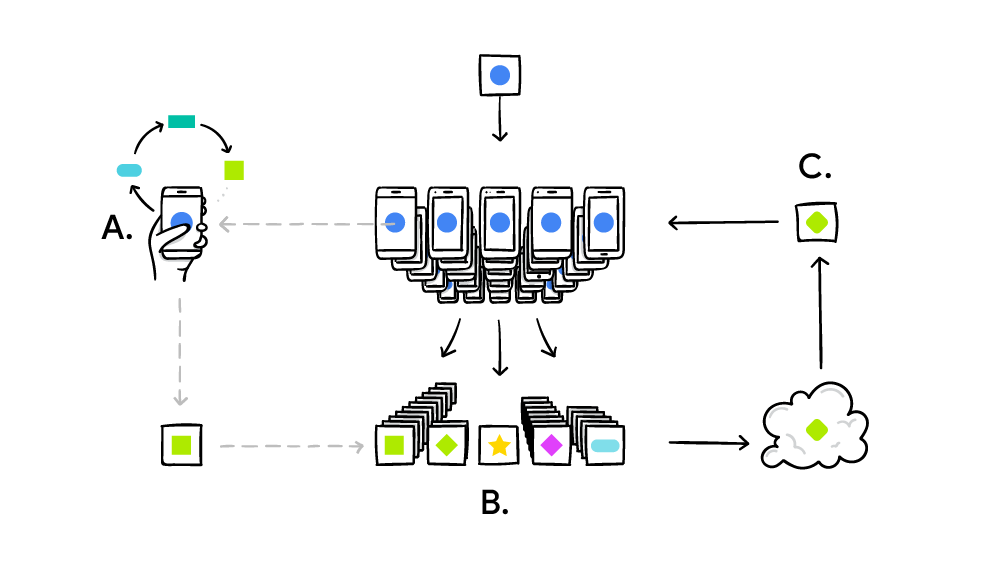
\includegraphics[keepaspectratio, scale=0.3]{federated-learning-flow.png}
	\caption{Federated Learningの流れ~\cite{mcmahan_ramage_2017}}
	\label{fig:federated-learning-flow}
\end{figure}

\end{frame}

\section{イントロダクション}

\begin{frame}{システムの概要}

\begin{itemize}
	\item システムの概要
	\begin{itemize}
		\item モバイル端末(Androidのスマートフォン)を対象としたシステム
		\newline
		\item スケーラブルかつ、実際の製品にもデプロイ可能なレベル \\
		$\Leftarrow$ Gboard(Google Keyboard)というキーボードアプリで実際に使用
		\newline
		\item 実装には、TensorFlowが用いられている \\
		$\Leftarrow$ 深層ニューラルネットの学習も可能である
		\newline
		\item 同期型の訓練アルゴリズム(\alert{Federated Averaging})を採用
		\item セキュリティ向上のための手法(\alert{Secure Aggregation})を利用可能
	\end{itemize}
\end{itemize}

\end{frame}

\begin{frame}{同期型の訓練アルゴリズム}

\begin{itemize}
	\item \alert{同期型}の訓練アルゴリズムが採用された
	\begin{itemize}
		\item 具体的には、\alert{Federated Averaging}というアルゴリズムを使用 \\
		$\Leftarrow$ SGD(Stochastic Gradient Descent)とよく似ている \\
		$\Leftarrow$ SGDを、重み付きの更新によって拡張したような手法
	\end{itemize} \
	
	\item クラウド上のモデルが更新されるまでの流れ
	\begin{enumerate}
		\item 各デバイスから、差分データ(モデルのパラメータの更新情報)を受信
		\newline
		\item \alert{Federated Averaging}を用いて、クラウド上で差分データを一つに集約
		\newline
		\item 集約された差分を、モデルのパラメータに反映(モデルの更新)
		\newline
		\item 更新されたモデルを、各デバイスが取得できるようになる
	\end{enumerate}
\end{itemize}

\end{frame}

\begin{frame}{同期型の訓練アルゴリズム}

\begin{itemize}
	\item \alert{同期型}の訓練アルゴリズムが採用された
	\begin{enumerate}
		\item 近年、同期型の訓練アルゴリズムを採用する動きがみられるため \\
		$\Leftarrow$ 同期処理の負担が大きなデータセンタですら、同期型の訓練アルゴリズムを採用する傾向
		\newline
		
		\item プライバシーを強化する手法を適用するため \\
		$\Leftarrow$ Differential PrivacyやSecure Aggregationなどの手法がある \\
		$\Leftarrow$ これらは原則として、同期型のアルゴリズムでないと適用不可能
		\newline
		
		\item サーバ側での処理が単純になるため \\
		$\Leftarrow$ 多数のユーザ(デバイス)からの更新データをまとめて、モデルに適用
	\end{enumerate} \
	
	\begin{itemize}
		\item 但し、同期処理のオーバヘッドを軽減するための対策が必要(後述)
	\end{itemize}
\end{itemize}

\end{frame}

\begin{frame}{セキュリティ向上のための手法}

\begin{itemize}
	\item セキュリティ向上のための手法を利用可能
	\begin{itemize}
		\item 具体的には、\alert{Secure Aggregation}という手法を利用可能 \\
		$\Leftarrow$ 各デバイスから送信される差分データは、外部から隠される
		\newline
		
		\item Federated Learningでは、訓練データは各デバイス上に留まる \\
		$\Leftarrow$ 訓練データには、個人を特定するに足る情報が含まれるかもしれない \\
		$\Leftarrow$ クラウド上にデータを保存しないことで、プライバシーが確保される
		\newline
		
		\item データは送信しない代わりに、データを元に算出した差分データを送信 \\
		$\Leftarrow$ 差分データには、各デバイスを特定するのに十分な情報が、依然として含まれる可能性 \\
		$\Leftarrow$ 差分データをも隠蔽することで、セキュリティを更に向上させられる
	\end{itemize}
\end{itemize}

\end{frame}

\begin{frame}{システムを実装する上での課題}

\begin{itemize}
	\item システムを実装する上での課題が非常に多い
	\begin{enumerate}
		\item デバイスが常に接続されているとは限らない \\
		$\Leftarrow$ デバイス(スマートフォン)の接続状態は不安定になりがち
		\newline
		
		\item デバイスが常に計算可能とは限らない \\
		$\Leftarrow$ 計算が途中で中断させられるかもしれない \\
		$\Leftarrow$ デバイスは世界中に散らばって存在するため、地理的な要因(タイムゾーンなど)を考慮する必要がある
		\newline
		
		\item 複数のデバイスの同期処理を取るのが困難 \\
		$\Leftarrow$ 前述の通り、これらのデバイスは接続状態が不安定で、常に利用できるかどうかも分からない
		\newline
		
		\item デバイスの計算能力とストレージの制限が厳しい \\
		$\Leftarrow$ 深層ニューラルネットの場合はパラメータ数が多く、メモリと計算資源の消費が特に大きい
	\end{enumerate}
\end{itemize}

\end{frame}

\begin{frame}{システムを実装する上での課題}

\begin{itemize}
	\item これらの課題を3つの構成要素で解決
	\begin{itemize}
		\item \alert{通信プロトコル}、\alert{デバイス}、\alert{サーバ}
		\item この3つの動作について、これからみていく
		\newline
		
		\item 論文の著者によれば、このシステムは数百万、あるいは十億台のデバイス上で利用可能だとしている
	\end{itemize}
\end{itemize}

\end{frame}

% ここまでの話の流れ

\section{通信プロトコル}

\begin{frame}{通信プロトコルの用語整理}

\begin{itemize}
	\item プロトコルの主人公
	\begin{itemize}
		\item デバイス (ここではAndroidのスマートフォン)
		\item \alert{FL Server} (クラウドベースの分散サービス)
	\end{itemize} \
	
	\item \alert{FL Population}
	\begin{itemize}
		\item 学習アルゴリズムで解こうとしている問題
	\end{itemize} \
	
	\item \alert{FL Task}
	\begin{itemize}
		\item 特定の計算タスク \\
		$\Leftarrow$ あるハイパーパラメータが与えられた下での学習 \\
		$\Leftarrow$ デバイス上のローカルなデータを用いた、モデルの評価
		\newline
		\item FL Populationは、複数のFL Taskによって構成される \\
		$\Rightarrow$ FL Taskは、必ず何らかのFL Populationに属する
	\end{itemize}
\end{itemize}

\end{frame}

\begin{frame}{通信プロトコルの用語整理}

\begin{itemize}
	\item \alert{FL Plan}
	\begin{itemize}
		\item TensorFlowの計算グラフや、タスクの実行方法を格納するデータ構造
	\end{itemize} \
	
	\item \alert{FL Checkpoint}
	\begin{itemize}
		\item クラウド上の現在のモデルのパラメータ
		\item その他の状態 (シリアライズ化されたTensorFlowのセッション)
	\end{itemize} \
	
	\item \alert{Round}
	\begin{itemize}
		\item FL Serverとデバイスとの一連の通信(後述)
		\item \alert{Selection}、\alert{Configuration}、\alert{Reporting}の3段階で構成される
		\item 次の図\ref{fig:fl-protocol}を参照
	\end{itemize}
\end{itemize}

\end{frame}

\begin{frame}{Federated Learningのプロトコル}

\begin{figure}
	\centering
	\includegraphics[keepaspectratio, scale=0.6, clip, trim=2cm 15.5cm 2cm 2.5cm, page=2]{papers/Towards-Federated-Learning-at-Scale-1902-01046.pdf}
	\caption{Federated Learningのプロトコル~\cite{DBLP:journals/corr/abs-1902-01046}}
	\label{fig:fl-protocol}
\end{figure}

\end{frame}

\begin{frame}{Federated Learningのプロトコル}

\begin{itemize}
	\item Federated Learningのプロトコルの大まかな流れ
	\begin{enumerate}
		\item FL Serverは、ある決められた時間だけ、デバイスからの報告を待機 \label{enum:fl-protocol-begin} \\
		$\Leftarrow$ ある特定のFL Taskが実行可能であることの報告を待つ
		\newline
		\item 多数のデバイスが、指定されたFL Taskを実行可能であることを、FL Serverに伝達
		\newline
		\item FL Serverは、報告してきた数千のデバイスの中から、数百程度のデバイスを選択 \label{enum:fl-protocol-device-selection}
		\newline
		\item 選ばれた数百のデバイスで、FL Taskを実行する \label{enum:fl-protocol-end}
		\newline
		\item (\ref{enum:fl-protocol-begin})から(\ref{enum:fl-protocol-end})までを繰り返す \\
		$\Rightarrow$ この繰り返しの単位をRoundという \\
		$\Rightarrow$ (\ref{enum:fl-protocol-begin})から(\ref{enum:fl-protocol-device-selection})までが\alert{Selection}フェーズ \\
		$\Rightarrow$ (\ref{enum:fl-protocol-end})が\alert{Configuration}と\alert{Reporting}フェーズ
	\end{enumerate}
\end{itemize}

\end{frame}

\begin{frame}{Federated Learningのプロトコル}

\begin{itemize}
	\item Federated LearningのプロトコルのRoundの流れ
	\begin{itemize}
		\item Roundは\alert{Selection}、\alert{Configuration}、\alert{Reporting}の3段階で構成される
		\item Roundの間は、選択されたデバイスはFL Serverとの通信を継続する
		\newline
		
		\item Roundの実行途中で、時間内に応答しないデバイスは\alert{単に無視}される
		\item Federated Protocolのプロトコルは、このようなデバイスの脱落を考慮に入れて設計されている
	\end{itemize}
\end{itemize}

\end{frame}

\begin{frame}{Federated Learningのプロトコル}

\begin{itemize}
	\item Selectionフェーズの流れ
	\begin{enumerate}
		\item FL Taskの実行に適したデバイスは、周期的にFL Serverにアクセス \\
		$\Leftarrow$ \alert{充電中}で、かつ\alert{Wi-Fi}に接続されているデバイス \\
		$\Leftarrow$ 従量課金制のネットワークに接続されたデバイスは、アクセスしない(Federated Learningには参加しない)
		\newline
		
		\item FL Serverにアクセスしたデバイスは、双方向のコネクションを確立 \\
		$\Leftarrow$ Roundの間は、コネクションを維持する必要がある
		\newline
		
		\item FL Serverは、接続してきた数千のデバイスの中から、数百程度のデバイスを選択 \\
		$\Leftarrow$ 1つのRoundには数百程度のデバイスが参加 \\
		$\Leftarrow$ 選択に使用するアルゴリズムは何でもよい(溜池サンプリング)
		\newline
		
		\item 選ばれなかったデバイスに対して、FL Serverは次にアクセスすべき時刻を送信(適当な時間の経過後に、再接続させる)
	\end{enumerate}
\end{itemize}

\end{frame}

\begin{frame}{Federated Learningのプロトコル}

\begin{itemize}
	\item Selectionフェーズで指定可能なパラメータの例
	\begin{itemize}
		\item FL Taskの実行に協力して欲しいデバイスの数(希望)
		\item FL Taskの実行に最低限必要なデバイスの数(閾値)
		\item FL Serverがデバイスからの接続を待つべき時間(タイムアウト)
	\end{itemize} \
	
	\begin{itemize}
		\item 希望通りの数のデバイスが接続してきた時点で、Roundの実行が開始
		\item タイムアウトになるまでは、接続デバイス数が希望通りになるまで待機
		\newline
		\item タイムアウト時に、接続デバイス数が閾値を超えていなければ、Roundは実行されない
	\end{itemize}
\end{itemize}

\end{frame}

\begin{frame}{Federated Learningのプロトコル}

\begin{figure}
	\centering
	\includegraphics[keepaspectratio, scale=0.6, clip, trim=2cm 15.5cm 2cm 2.5cm, page=2]{papers/Towards-Federated-Learning-at-Scale-1902-01046.pdf}
	\caption{Federated Learningのプロトコル(再掲)~\cite{DBLP:journals/corr/abs-1902-01046}}
\end{figure}

\end{frame}

\begin{frame}{Federated Learningのプロトコル}

\begin{itemize}
	\item Configurationフェーズの流れ
	\begin{enumerate}
		\item 選択されたデバイスに対して、FL Planを送信 \\
		$\Leftarrow$ FL Planは、TensorFlowの計算グラフや、FL Taskの実行方法を格納
		\newline
		
		\item 続いて、選択されたデバイスに対して、FL Checkpointを送信 \\
		$\Leftarrow$ FL Checkpointは、モデルのパラメータや、FL Taskの実行に必要な様々な情報を格納 \\
		$\Leftarrow$ シリアライズ化されたTensorFlowのセッションオブジェクトなど
		\newline
		
		\item デバイスは、FL Serverから渡された情報を元に、FL Taskを実行 \\
		$\Leftarrow$ デバイス上に保存されたデータを用いた、モデルの訓練や評価
	\end{enumerate}
\end{itemize}

\end{frame}

\begin{frame}{Federated Learningのプロトコル}

\begin{itemize}
	\item Reportingフェーズの流れ
	\begin{enumerate}
		\item FL Serverは、デバイスから結果が送信されるのを待機 \\
		$\Leftarrow$ FL Taskがモデルの訓練であれば、差分データ(モデルのパラメータの更新情報)の送信を待機
		\newline
		
		\item FL Serverは、Federated Averagingを使って、差分データを一つに集約 \\
		$\Leftarrow$ 集約された差分を、モデルのパラメータに反映(モデルの更新)
		\newline
		
		\item FL Serverは、タスクを実行し終えたデバイスに対して、次にアクセスすべき時刻を送信 \\
		$\Leftarrow$ 適当な時間の経過後に、デバイスがFL Serverに再接続するように指示
	\end{enumerate} \
	
	\begin{itemize}
		\item 十分な数のデバイスが結果を報告すれば、モデルの更新が実行される
		\item それ以外の場合は、Roundの実行は失敗(無かったことにされる)
	\end{itemize}
\end{itemize}

\end{frame}

\begin{frame}{Federated Learningのプロトコル}

\begin{itemize}
	\item デバイスのFL Serverへの接続頻度の調節
	\begin{itemize}
		\item FL Population(解こうとしている問題)の大きさに応じて、デバイスの接続頻度(一度にFL Serverに接続してくるデバイス数)を調節
		\newline
		
		\item FL Serverは、次に再接続すべき時間を、各デバイスに対して指示する \\
		$\Rightarrow$ この時間をうまく調節することで、デバイスの接続頻度を調節可能
		\newline
		
		\item FL Taskに協力可能(\alert{アクティブ})なデバイスの数は、周期的に変動 \\
		$\Rightarrow$ 充電中で、かつWi-Fiに接続されていればアクティブとみなす \\
		$\Rightarrow$ 昼の時間帯は人間が使用するので、アクティブなデバイスが減少 \\
		$\Rightarrow$ それ以外の時間帯(深夜)では、逆にアクティブなデバイスが増加
		\newline
		
		\item これらの周期的な変動も考慮して、再接続までの時間を指定 \\
		$\Rightarrow$ 例えば、昼間の時間帯は、FL Serverにアクセスする頻度を落とす
	\end{itemize}
\end{itemize}

\end{frame}

\begin{frame}{Federated Learningのプロトコル}

\begin{itemize}	
	\item 小さなFL Populationの場合(解こうとしている問題が小さい)
	\begin{itemize}
		\item FL Taskに参加するデバイスの数も少なくて済む
		\newline
		
		\item 十分な数のデバイスが、FL Serverにほとんど同時に接続できるように、接続頻度を上手く調節する \\
		$\Rightarrow$ Selectionフェーズに掛かる時間が短縮 \\
		$\Rightarrow$ 単位時間に実行可能なRoundの数が増加 \\
		$\Rightarrow$ 学習が速やかに進行する
	\end{itemize}
\end{itemize}

\end{frame}

\begin{frame}{Federated Learningのプロトコル}

\begin{itemize}
	\item 大きなFL Populationの場合(解こうとしている問題が大きい)
	\begin{itemize}
		\item 一般的に、FL Taskに協力してくれるデバイスが多数存在する
		\item 但し、一度のRoundに参加するデバイスは、せいぜい数百程度である
		\newline
		
		\item 多数のデバイスが、一度にFL Serverに接続しないようにする \\
		$\Rightarrow$ 一度に多数のデバイスがFL Serverに接続しても、そのうちのごく一部のデバイスが選択され、他の多数のデバイスの接続が無駄になるかもしれない (\alert{Thundering Herd}と呼ばれる問題)
		\newline
		
		\item 各デバイスが、FL Serverにアクセスする時間を、ランダムに決める \\
		$\Rightarrow$ デバイスの接続を時間的に分散させる \\
		$\Rightarrow$ 必要なときに、必要な数のデバイスだけが接続する
	\end{itemize}
\end{itemize}

\end{frame}

\section{デバイス上のソフトウェア}

\begin{frame}{デバイス上のソフトウェア}

\begin{itemize}
	\item デバイス上のソフトウェア
	\begin{itemize}
		\item 今回のシステムは、Androidのスマートフォンが対象
		\item 但し、それ以外のプラットフォームでも実装可能
		\newline
		
		\item アプリケーションプロセス、\alert{FL Runtime}、\alert{Example Store}の3つが連携して動作
		\item 次の図\ref{fig:fl-device-arch}を参照
	\end{itemize}
\end{itemize}

\end{frame}

\begin{frame}{デバイス上のソフトウェアのアーキテクチャ}

\begin{figure}
	\centering
	\includegraphics[keepaspectratio, scale=0.8, clip, trim=10.5cm 15.5cm 2cm 5.5cm, page=3]{papers/Towards-Federated-Learning-at-Scale-1902-01046.pdf}
	\caption{デバイス上のソフトウェアのアーキテクチャ~\cite{DBLP:journals/corr/abs-1902-01046}}
	\label{fig:fl-device-arch}
\end{figure}

\end{frame}

\begin{frame}{デバイス上のソフトウェア}

\begin{itemize}
	\item \alert{Example Store}
	\begin{itemize}
		\item Federated Learningで使用するデータを保存しておくデータベース
		\item クラウド上にあるモデルの学習と、改良に用いられる訓練データ
		\newline
		
		\item 以下のような推奨事項がある
	\end{itemize}
	
	\begin{enumerate}
		\item ストレージを圧迫しないように、データベースの最大容量を、予め決めておく
		\item 各データの保存期間を決めておき、期間を過ぎたデータが自動的に削除されるようにする
		\item マルウェアによる不正アクセスを防止するため、各データを適切に暗号化しておく
	\end{enumerate}
\end{itemize}

\end{frame}

\begin{frame}{デバイス上のソフトウェア}

\begin{itemize}
	\item \alert{FL Runtime}
	\begin{itemize}
		\item FL Serverとのやり取りを行うソフトウェアのコンポーネント
		\newline
		
		\item FL Taskを実行する際、Example Storeからデータを取得
		\item 取得したデータを用いて、FL Taskで指定された処理(モデルの訓練や評価)を実行する
	\end{itemize}
\end{itemize}

\end{frame}

\begin{frame}{参考文献}

\bibliographystyle{plain}
\bibliography{federated-learning-bibliography}

\end{frame}

\end{document}
